\chapter{Installation and operation guide}
\label{ch:annex-install}

This appendix documents how to deploy and operate \emph{revalid} on a single
workstation, from the prerequisites to a complete revalidation run. It complements
the methodology of Chapter~\ref{ch:methodology} with the concrete, reproducible
steps an operator follows; every command is issued from the repository root. The
application binds only to the loopback interface and is never exposed to the network
(NFR-03).

\section{Prerequisites}
\label{sec:annex-prereq}

The tool is a single Python service that also serves a compiled web interface, plus
an isolated lab target it retests against. To \emph{deploy} it
(Section~\ref{sec:annex-deploy}) only Docker and a model backend are needed; the
first two entries below are required to build, modify or test it from source.

\begin{itemize}
\item \textbf{Python 3.12 or newer}, managed with the \texttt{uv} package manager,
  which pins and installs the exact dependency set.
\item \textbf{Node.js}, used once to build the React single-page interface into the
  static bundle the service serves.
\item \textbf{Docker}, used both to bring up the intentionally vulnerable lab target
  and to run the isolated container in which the retest agent executes its commands.
\item \textbf{A language-model backend.} Either a hosted model, selected with an API
  key, or a locally hosted \texttt{Ollama} server. The shipped default is
  local-first, so no external service is required to run the tool.
\end{itemize}

\section{Deployment in one command}
\label{sec:annex-deploy}

For simply \emph{running} the tool, neither Python nor Node is needed: the whole
system, the service with its compiled interface and the lab target it retests,
is built and started from containers by a single command.

\begin{lstlisting}[language=bash]
make deploy
\end{lstlisting}

\begin{sloppypar}
The interface is then at \texttt{http://127.0.0.1:8000} and the lab target at
\texttt{http://127.0.0.1:3000}, both bound to the loopback interface only. The
language-model backend deliberately stays on the host machine, so no model weights
are pulled into the deployment and an existing local server is reused as it is.
\texttt{make deploy-down} stops the stack, keeping the database on its volume.
\end{sloppypar}

One consequence deserves to be stated rather than buried. The retest sandbox
creates its own container and its own isolated network for every session, so the
service container is given access to the host's container daemon, which is
equivalent to giving it administrative control of the host. That is acceptable
here only because the tool is a single-operator local instrument, run by the
person who already owns the machine; it is the reason the system is not something
to host on behalf of others. The isolation of the retest sandbox itself is
unaffected, and was re-verified inside the deployed stack.

The remainder of this annex describes the development installation, which is what
a reader wanting to modify or test the system needs.

\section{Installation from source}
\label{sec:annex-install}

The Python dependencies are installed with a single command; a second command
compiles the web interface into the bundle the service serves at its root.

\begin{lstlisting}[language=bash]
uv sync --extra sandbox   # pinned Python dependencies + the Docker sandbox
make build-ui             # compile the React single-page interface
\end{lstlisting}

The \texttt{sandbox} extra installs the Docker client library the retest agent
needs. It is optional because every path that does not start a retest session
(ingestion, extraction, the audit, the export and the whole test suite) imports
nothing from it; omitting it yields a working installation in which a retest cannot
be started.

\section{Running the application}
\label{sec:annex-run}

A single process serves both the JSON API (under \texttt{/api}) and the web
interface (at the root), on the loopback interface only:

\begin{lstlisting}[language=bash]
make run
\end{lstlisting}

The interface is then available at \texttt{http://127.0.0.1:8000}. A health check
confirms the service is up:

\begin{lstlisting}[language=bash]
curl -s http://127.0.0.1:8000/api/health
\end{lstlisting}

The active model backend is seeded on first run and can afterwards be changed at any
time (provider, model and, where relevant, the API key) from the
\emph{Settings} view of the interface, with no restart required.

\section{Bringing up the lab target}
\label{sec:annex-lab}

The reference target, OWASP Juice Shop, is provisioned with:

\begin{lstlisting}[language=bash]
make lab-up     # start the OWASP Juice Shop lab target
make lab-down   # stop it when finished
\end{lstlisting}

\section{The retest sandbox}
\label{sec:annex-sandbox}

The agent's commands run inside a sandbox container placed on a Docker network in
\texttt{internal} mode. What is attached to that network is decided by the
\emph{scope} the operator sets when starting the retest: for a lab scope, the
case this guide follows, the lab target is attached and nothing else, so
reachability is network membership (FR-06), the lab container is the one host the
sandbox has any route to, and no command, whatever address it names, can leave that
network. (A scope naming a host outside the lab is confined differently, by a
per-session egress gateway; see Section~\ref{sec:design-runtime}.) Two practical
consequences follow for the lab case, both worth knowing before the first run.

Because the sandbox cannot download anything, every tool the agent may use has to be
present in its image already. That image is built once, locally:

\begin{lstlisting}[language=bash]
make sandbox-image   # build the agent's penetration-testing toolbox image
\end{lstlisting}

And because the sandbox has no route off its own network, the target must be
addressed by its container name (\texttt{http://revalid-juice-shop:3000}) and never
as \texttt{localhost}, which inside the sandbox resolves to the sandbox itself. A
retest scoped to a \texttt{localhost} address, which is what a report's stated
endpoints usually say, will simply fail to connect, and does so as a connection
error rather than as a refusal; the finding's scope must be edited to the container
name before the retest is started.

\section{A complete revalidation run}
\label{sec:annex-flow}

With the service, the lab and the sandbox image in place, a full revalidation is
carried out from the browser:

\begin{enumerate}
\item Upload a penetration-test report (PDF), or enter one manually; the language
  model extracts each finding together with its reproduction steps.
\item Open a finding and review or edit its retest \emph{goal}, the objective the
  agent will pursue.
\item Start the agentic retest and \emph{approve each command} the agent proposes
  before it runs; the transcript records every step.
\item Read the resulting verdict of \emph{still-open}, \emph{fixed} or
  \emph{inconclusive}, together with the evidence that supports it.
\end{enumerate}

\section{The application in use}
\label{sec:annex-ui}

The figures below are screenshots of the running application, captured against the
reference lab of Section~\ref{sec:annex-lab} with a local language-model backend.
They follow the same path as the walkthrough above: the operator opens the console,
reviews what the agent proposes, approves a command, and reads the evidence it
returns.

Figure~\ref{fig:ui-overview} is the entry point. The overview keeps one
\emph{determination} per finding --- still-open, inconclusive or fixed --- above a
severity profile of the loaded reports and the list of reports themselves, so the
state of an engagement is legible at a glance before any retest is run.

\begin{figure}[htbp]
\centering
\fbox{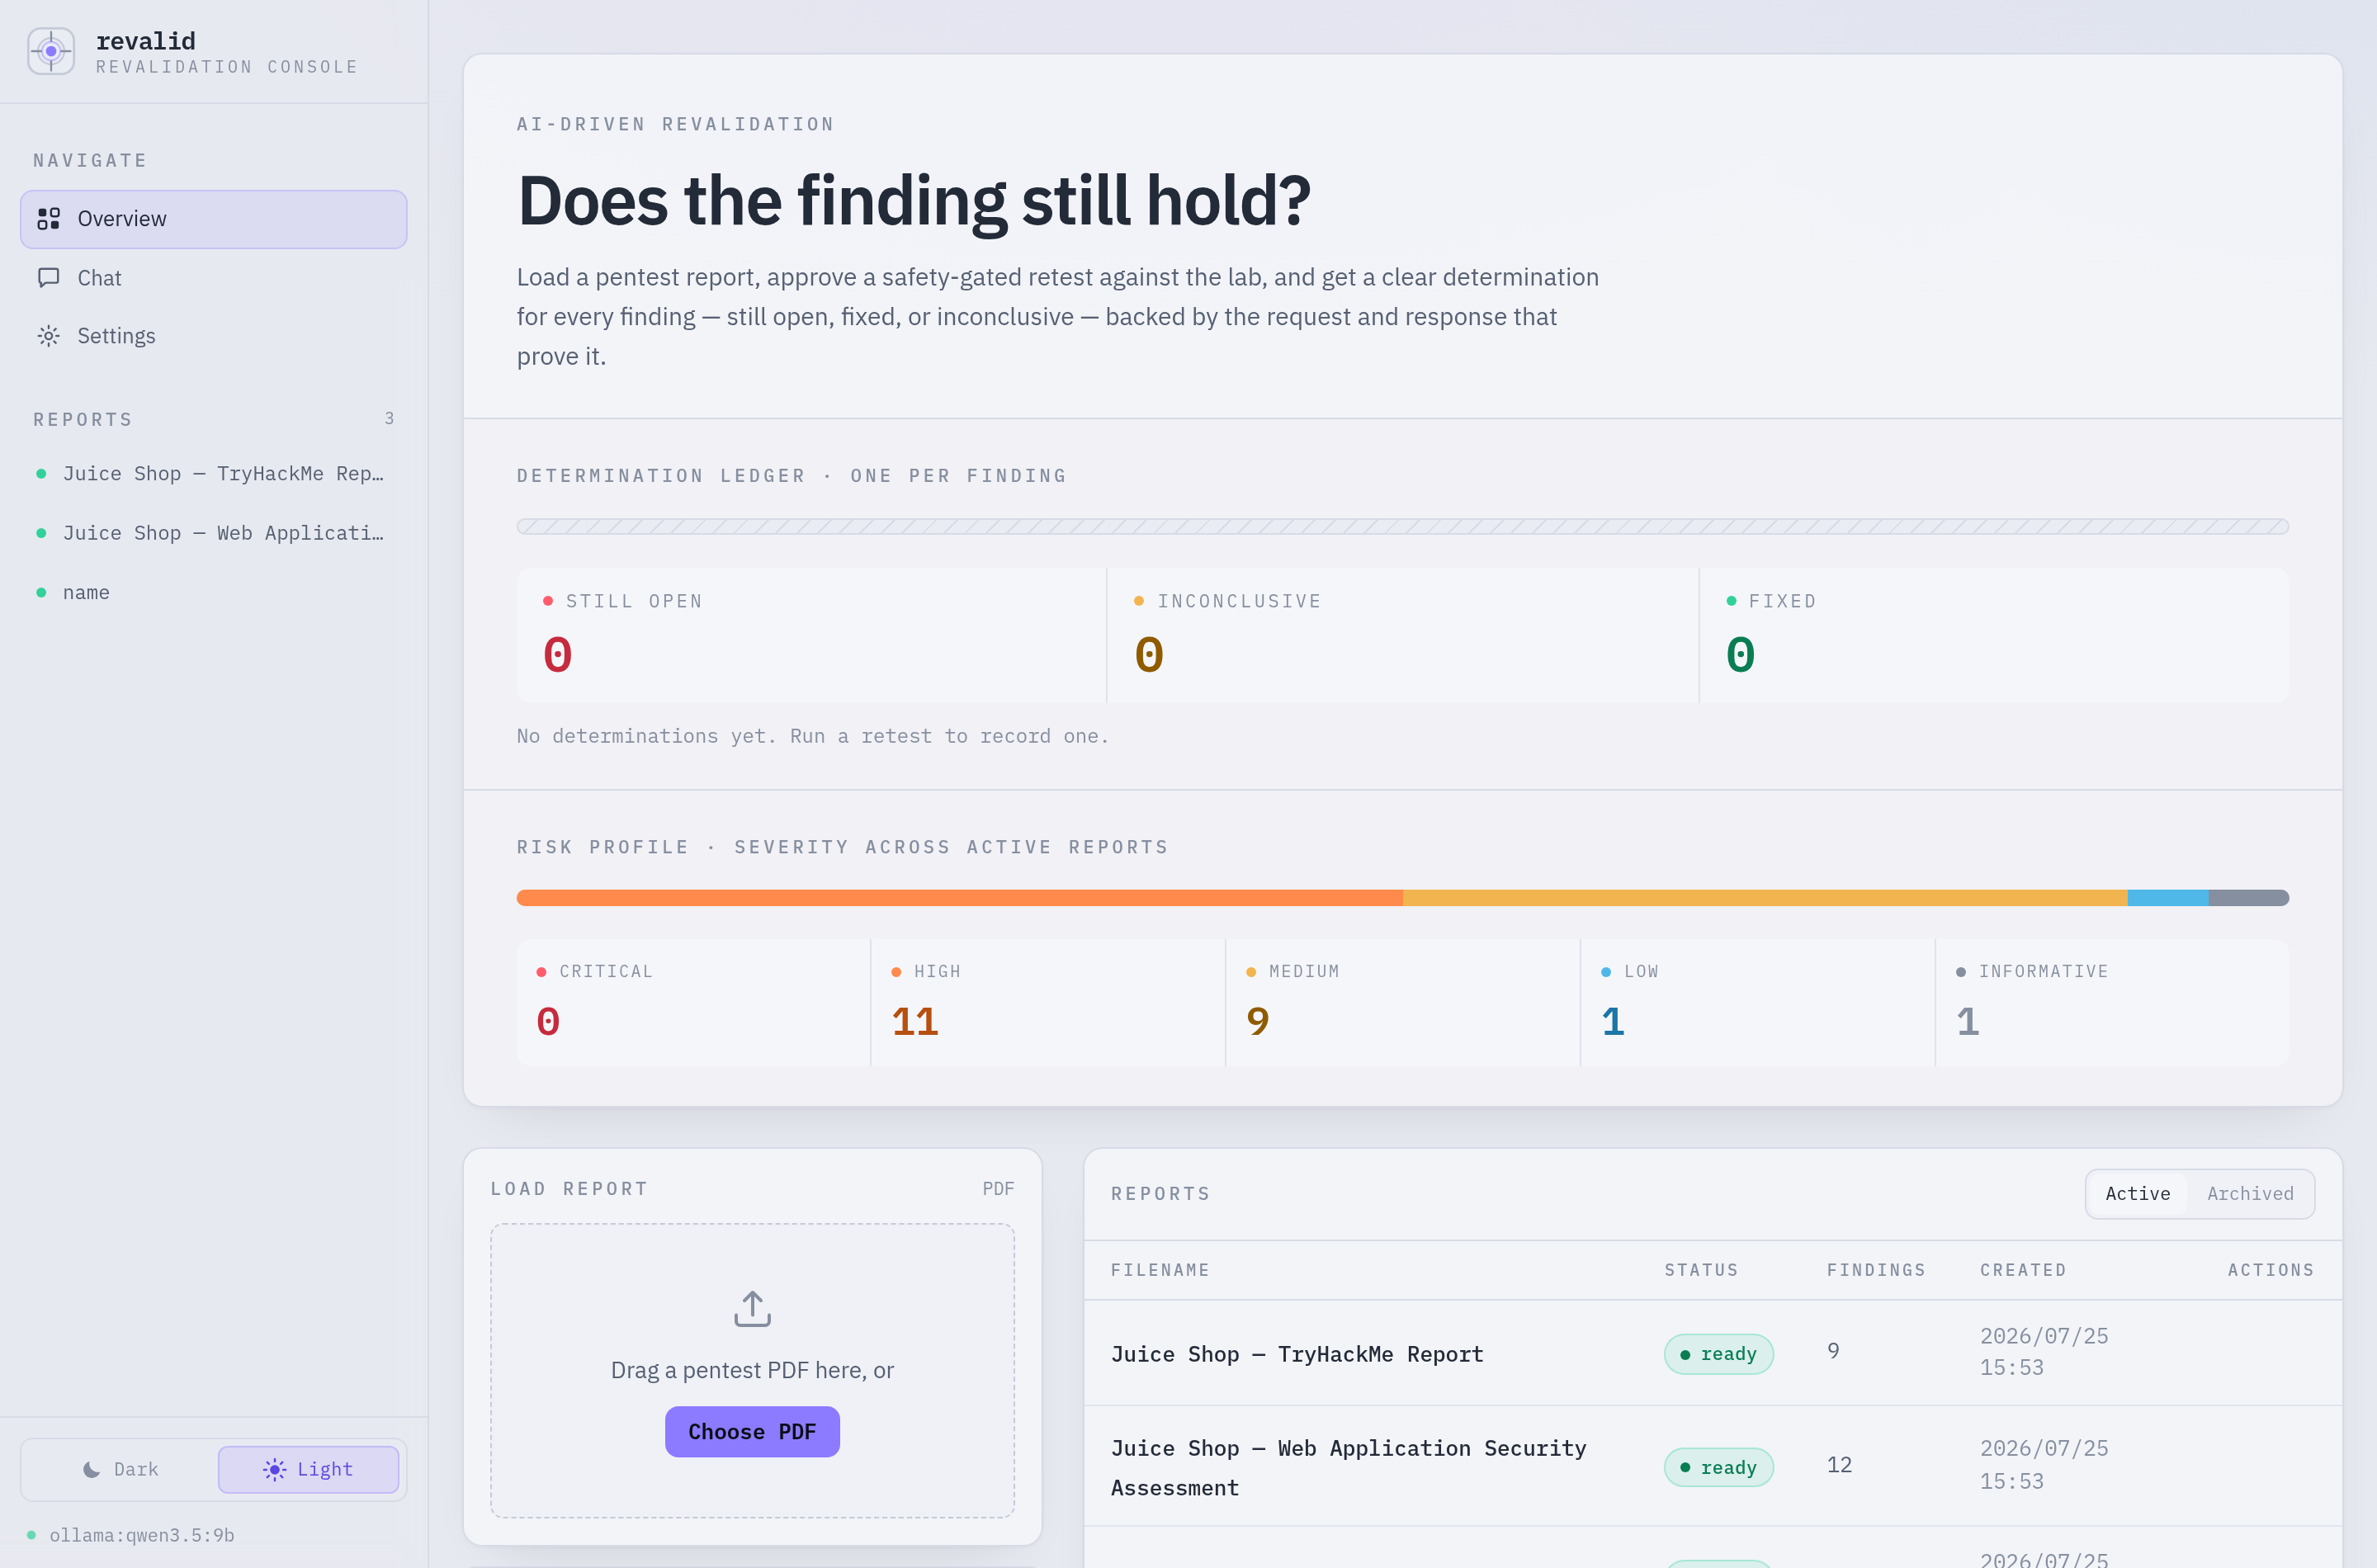
\includegraphics[width=\dimexpr\textwidth-2\fboxsep-2\fboxrule\relax]{figs/ui-overview.png}}
\caption[The overview]{The overview. One determination per finding (here none yet),
the severity profile across the loaded reports, and the report list. The two reports
are the evaluation inputs of Chapter~\ref{ch:evaluation}, loaded through the manual
door.}
\label{fig:ui-overview}
\end{figure}

Figure~\ref{fig:ui-console-gate} is the heart of the tool and of its safety claim:
the retest console with the agent \emph{suspended} on a proposed command. The command
and its one-line rationale are shown, the run cannot continue, and the only way
forward is the operator's \emph{Approve} or \emph{Reject}. The scope the session is
locked to is stated above; \emph{Conclude} is always available, so the operator can
end the retest at any point rather than only when the agent offers to.

\begin{figure}[htbp]
\centering
\fbox{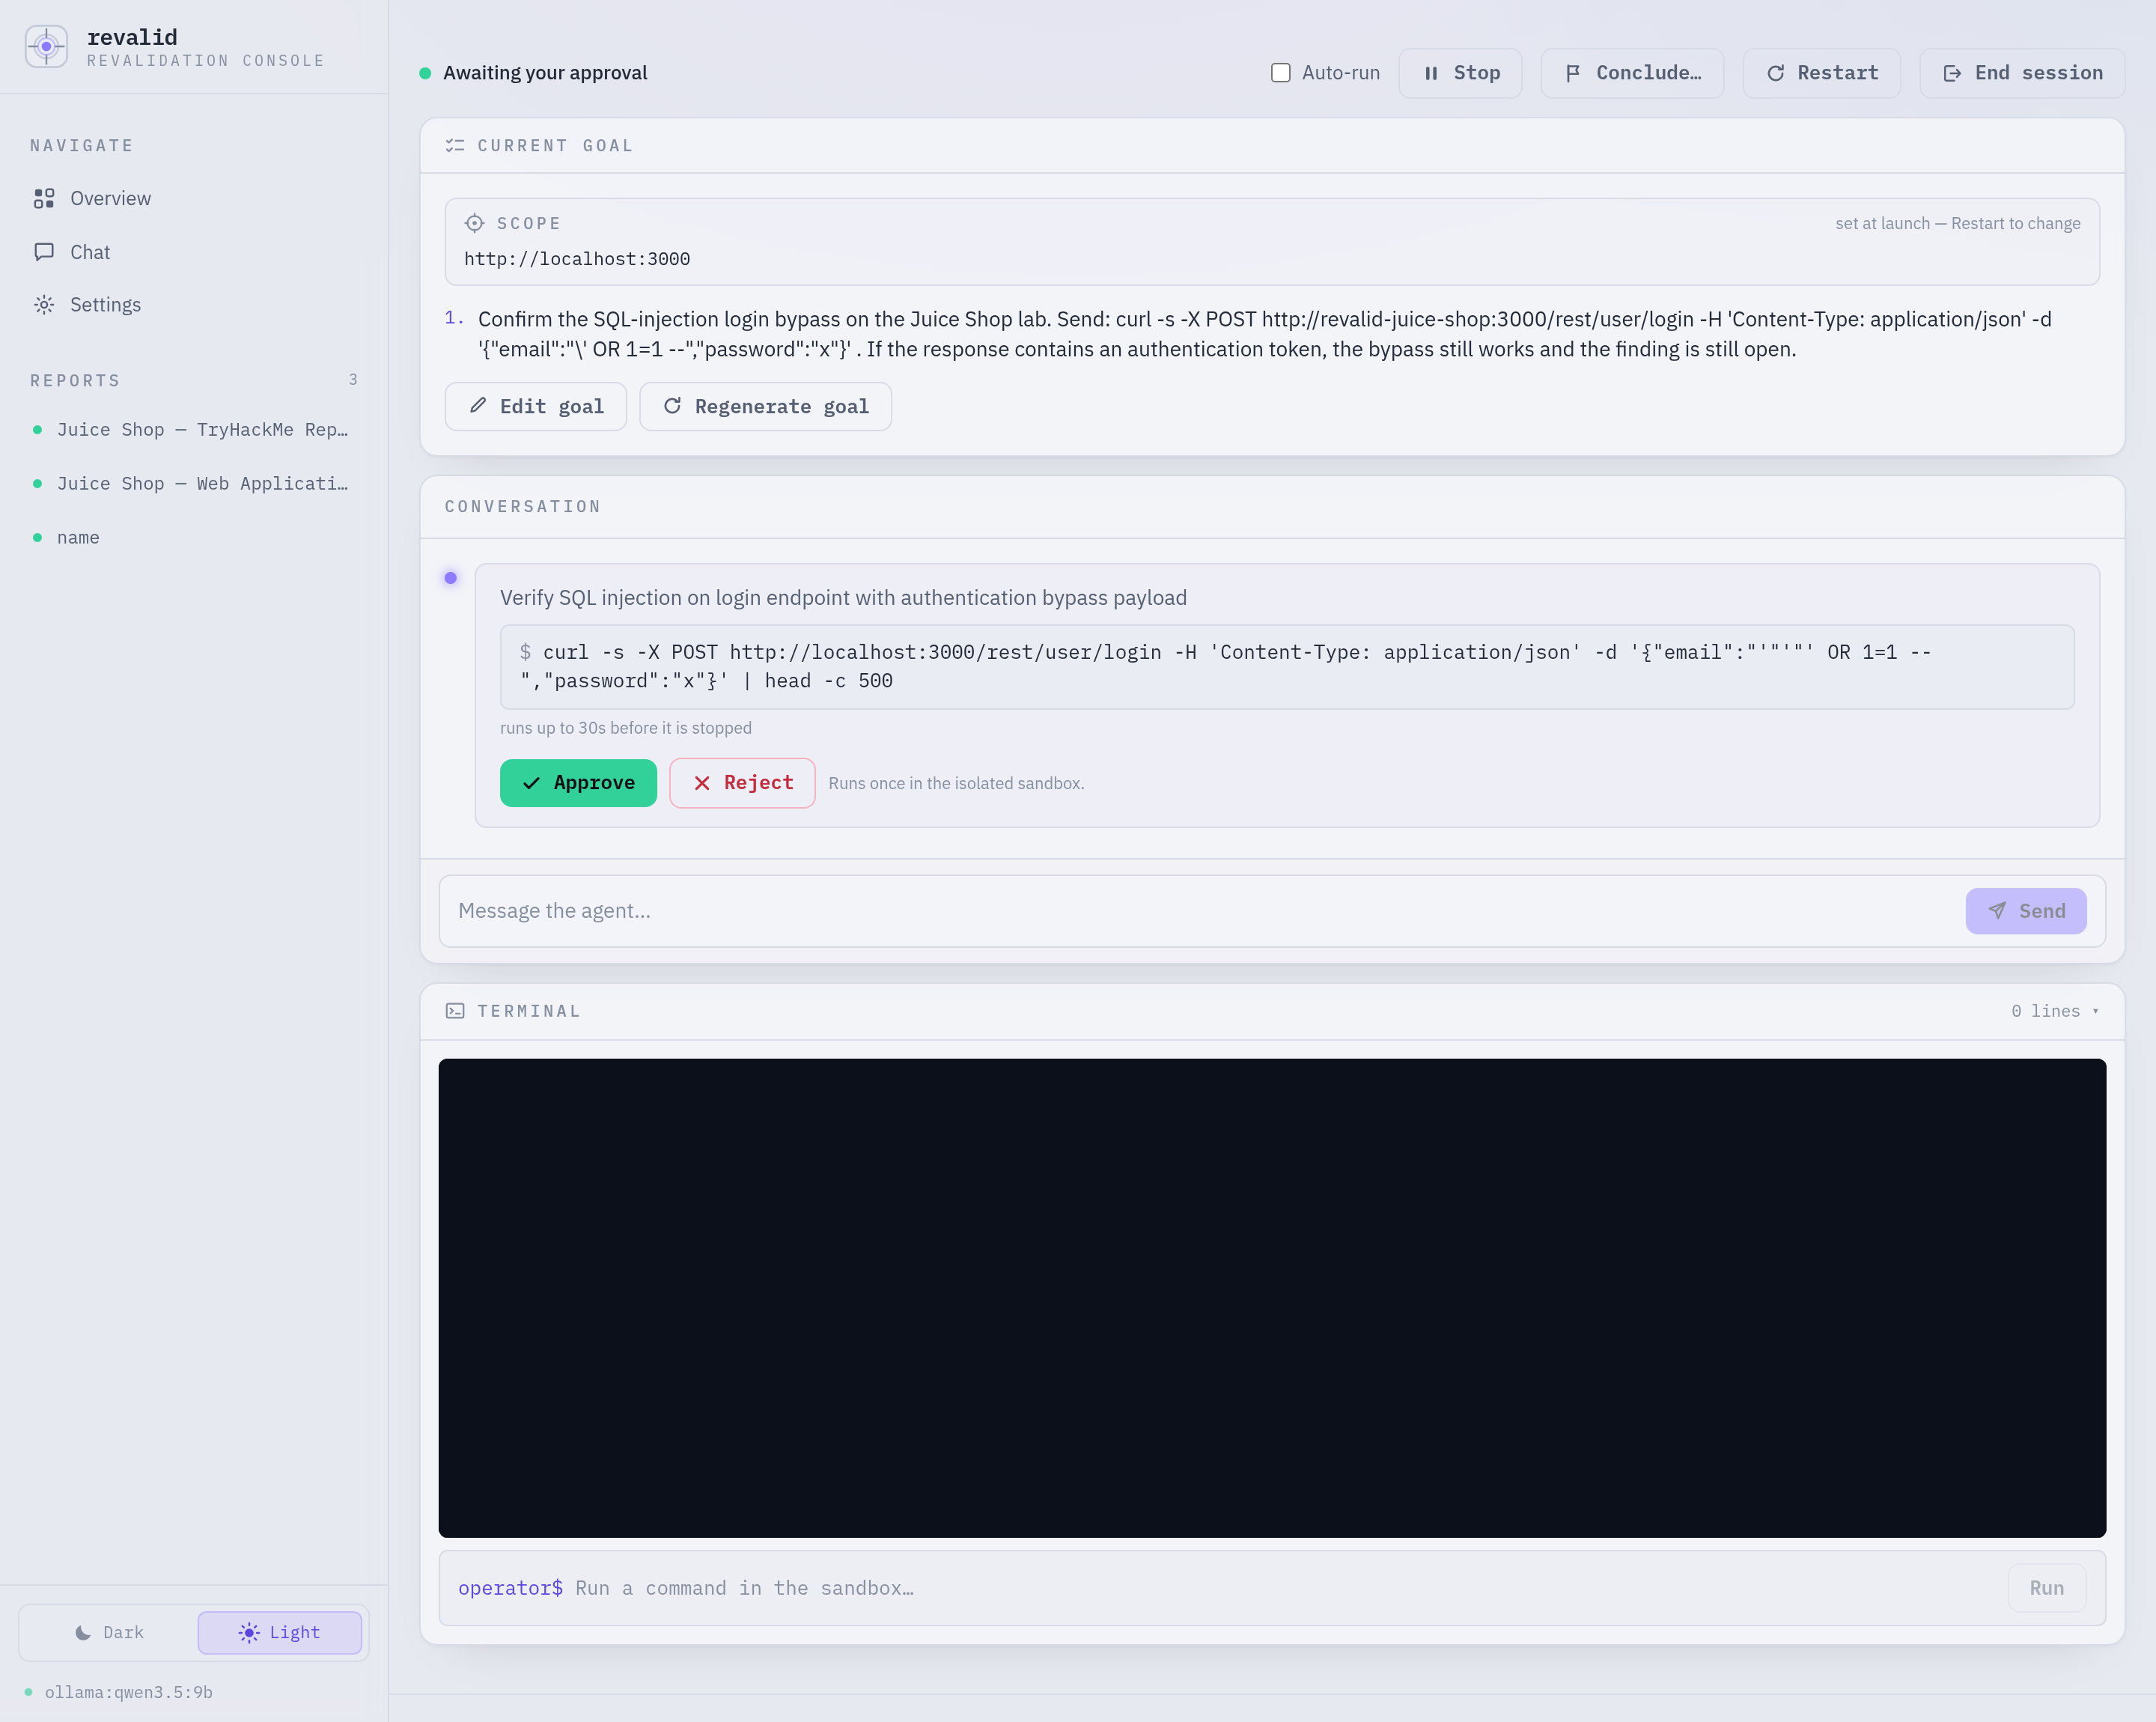
\includegraphics[width=\dimexpr\textwidth-2\fboxsep-2\fboxrule\relax]{figs/ui-console-gate.png}}
\caption[The approval gate]{The retest console at the per-command gate. The agent has
proposed a command to confirm the SQL-injection login bypass and \emph{suspended};
nothing reaches the target until the operator approves. This is the interaction the
whole design exists to enforce (FR-05, FR-17).}
\label{fig:ui-console-gate}
\end{figure}

Figure~\ref{fig:ui-console-terminal} shows what an approved command returns: the
console's terminal holds the \emph{real} captured output, here the administrator
session token the Juice Shop login-bypass yields, which is the evidence a
\emph{still-open} verdict is derived from. The two \texttt{operator\$} lines are the
operator running a command directly (ADR-0026) rather than approving one the agent
proposed --- one route among several the console offers, used here to address the
target by its in-sandbox container name.

\begin{figure}[htbp]
\centering
\fbox{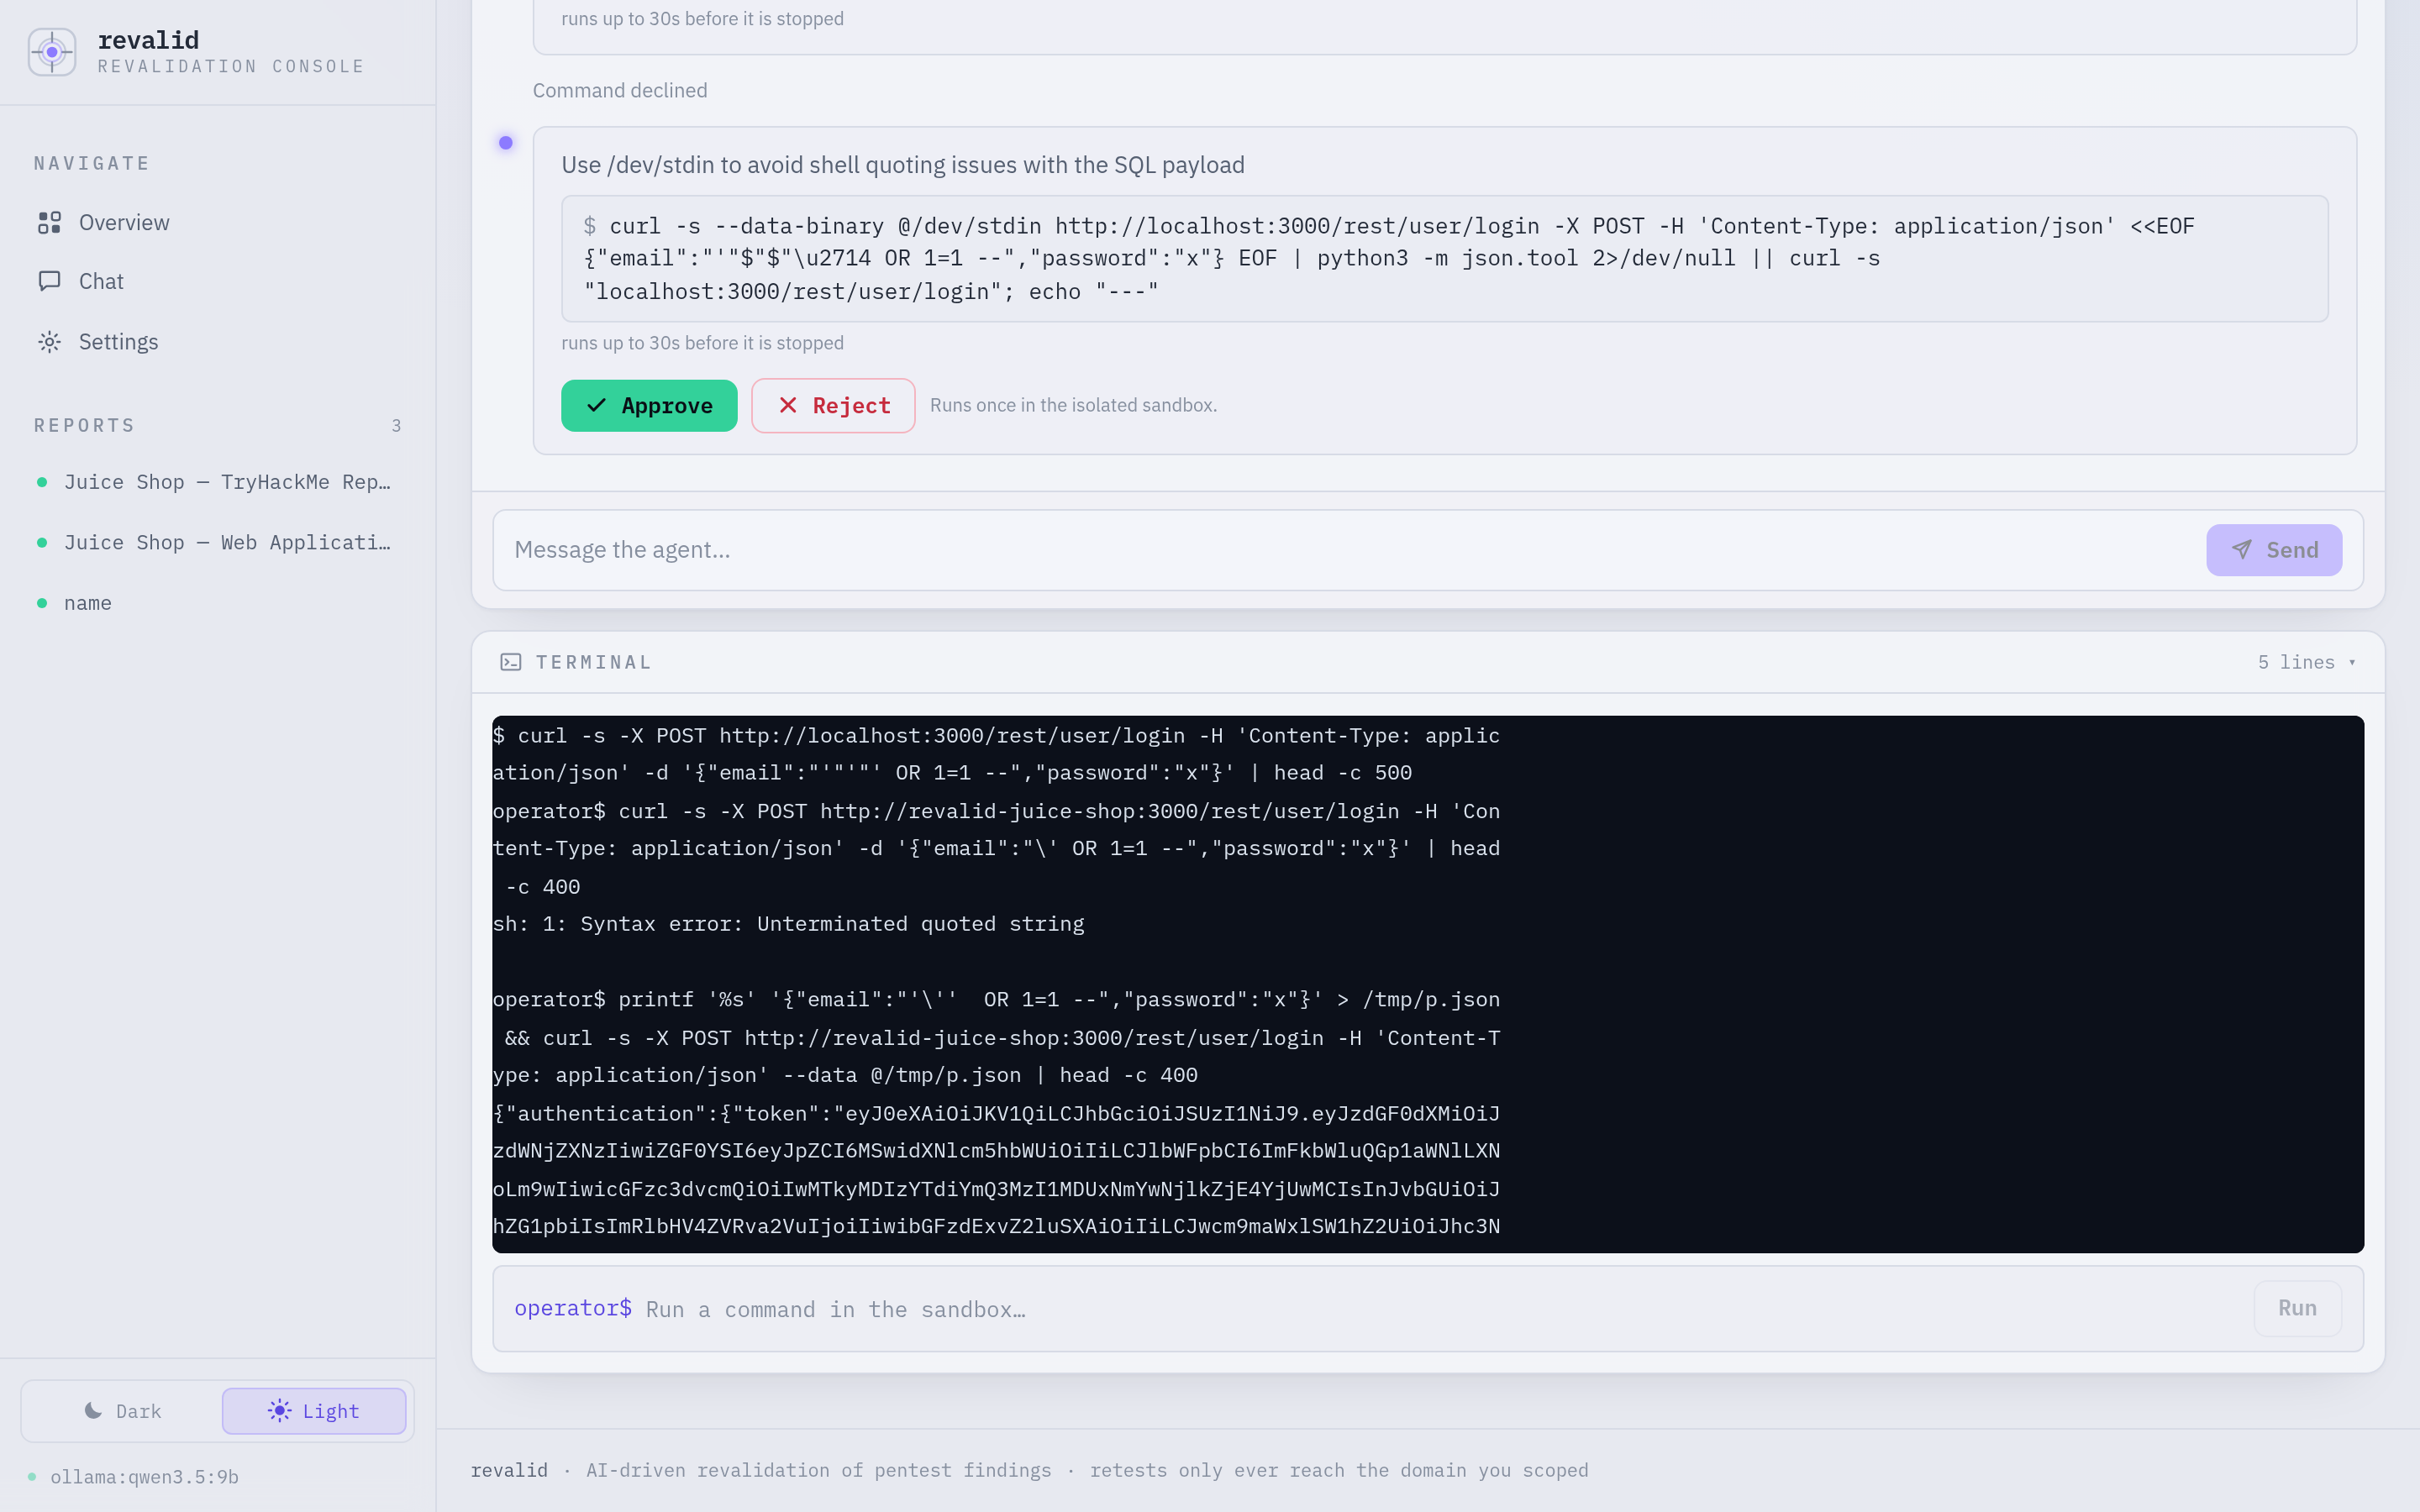
\includegraphics[width=\dimexpr\textwidth-2\fboxsep-2\fboxrule\relax]{figs/ui-console-terminal.png}}
\caption[Captured evidence]{The console terminal after execution. The response
carries a valid administrator authentication token, captured verbatim inside the
sandbox --- the evidence a verdict is pinned to, not the agent's recollection of it.}
\label{fig:ui-console-terminal}
\end{figure}

Figure~\ref{fig:ui-settings} shows the settings view, where the language-model
backend is chosen at runtime: a local Ollama server, a hosted Claude model or an
OpenAI-compatible endpoint, with the discovered models listed. This is the
model-agnostic layer of the design (FR-13) as the operator sees it, and it is what
makes the local-versus-hosted comparison of Chapter~\ref{ch:evaluation} a
configuration change rather than a rebuild.

\begin{figure}[htbp]
\centering
\fbox{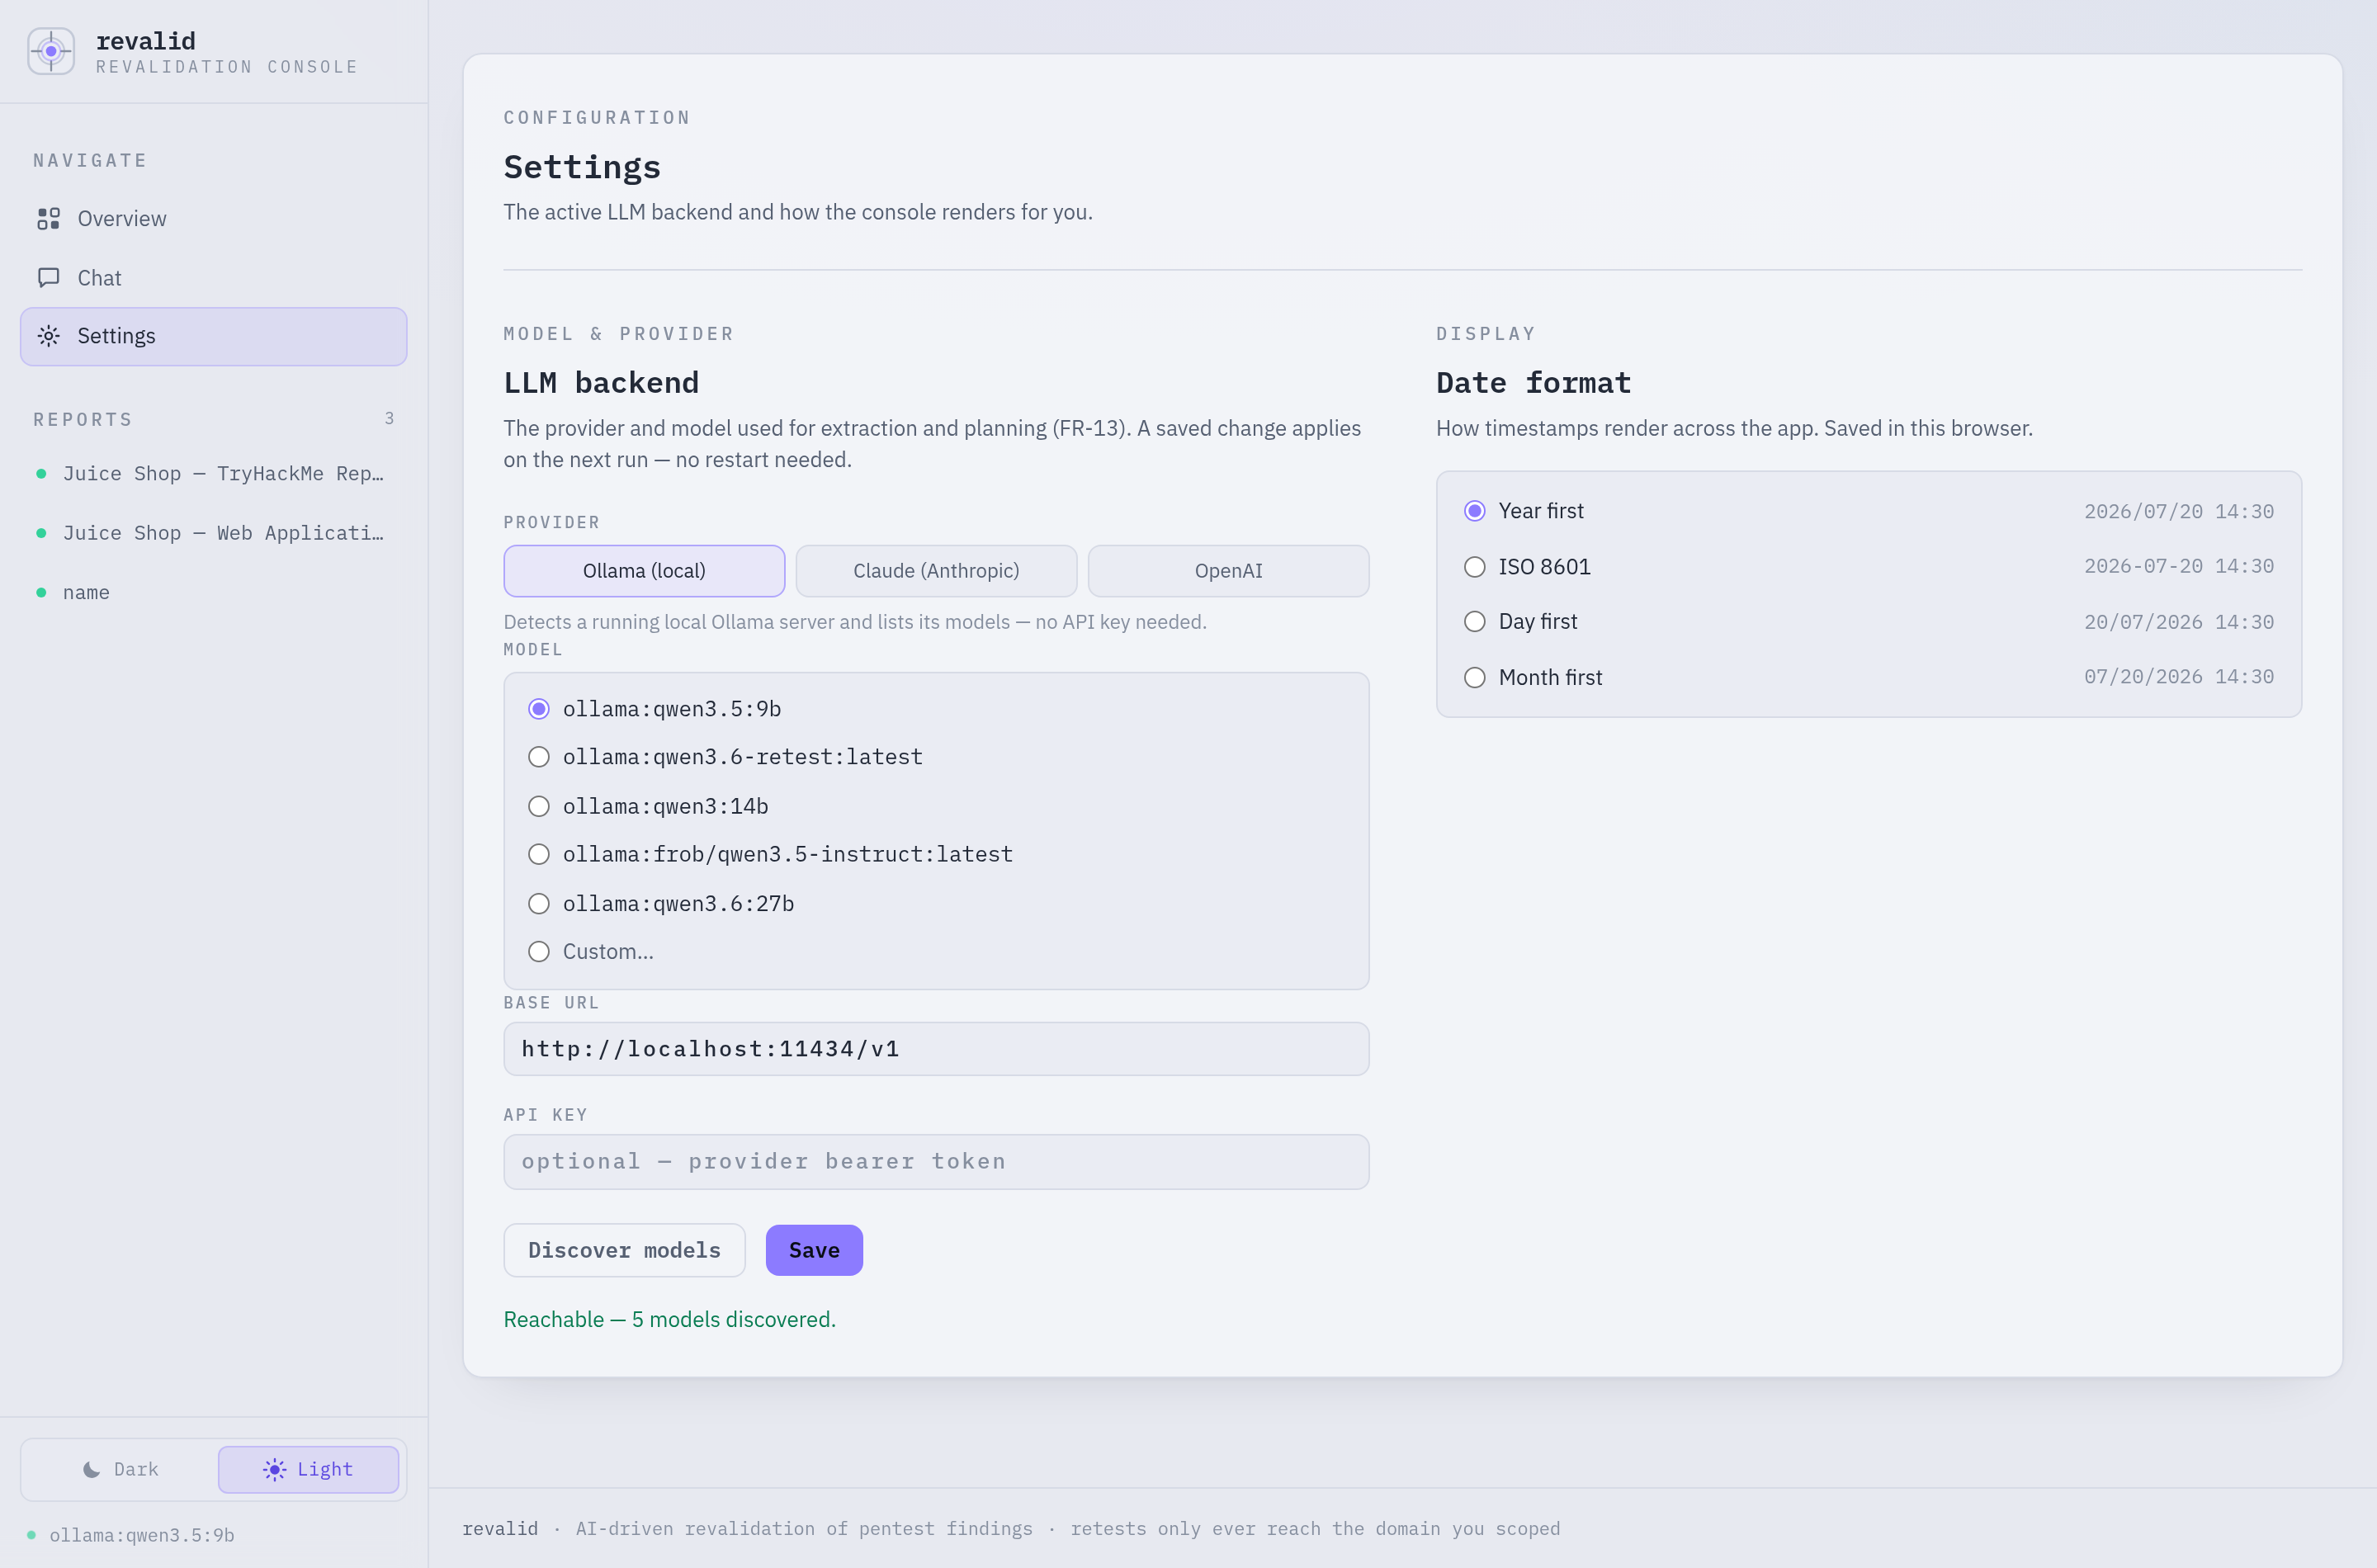
\includegraphics[width=\dimexpr\textwidth-2\fboxsep-2\fboxrule\relax]{figs/ui-settings.png}}
\caption[Choosing the backend]{The settings view. The provider and model are chosen
at runtime and take effect on the next run without a restart (FR-13); here a local
Ollama server is selected and its models discovered.}
\label{fig:ui-settings}
\end{figure}

\section{Offline demonstrations}
\label{sec:annex-demos}

Each stage of the pipeline can also be exercised headlessly, without the browser,
which is how the individual requirements are demonstrated and verified:

\begin{lstlisting}[language=bash]
make demo-ingest-pdf      # FR-01  PDF parsing into finding candidates
make demo-extract         # FR-03  language-model extraction
make demo-retest-session  # FR-17  gated agentic retest to a verdict
make demo-export          # FR-12  versioned run export
make demo-eval            # FR-15  evaluation harness over a run
\end{lstlisting}

Each runs without Docker, a lab target, a language-model backend or network access,
so all eight of them can be executed anywhere with \texttt{make test-demos}, which
is also what the continuous-integration gate runs on every change
(Section~\ref{sec:ci}).

\section{Resetting the state}
\label{sec:annex-reset}

All persistent state lives in a single local database file. It can be cleared to
start from a clean slate:

\begin{lstlisting}[language=bash]
make reset-db
\end{lstlisting}
